%This is a experiment example of ZhengXiaoyang's experiment report template

\documentclass[UTF8]{ctexart}

\usepackage{booktabs}
\usepackage{amsmath}
\usepackage{cases}
\usepackage{cite}
\usepackage{xeCJK}
\usepackage{graphicx}
\usepackage{SIunits}
\usepackage{caption}
\usepackage{float}
\usepackage{fancyhdr}
\usepackage[margin=1in]{geometry}
\geometry{a4paper}
\pagestyle{fancy}
\fancyhf{}

\graphicspath{{picture/}}


\title{拉脱法测量液体的表面张力系数}
\graphicspath{{picture/}}


\title{拉脱法测量液体的表面张力系数实验报告}
\author{郑晓旸}
\date{\today}
\pagenumbering{arabic}

\begin{document}
%这里是文件的开头
\fancyhead[L]{郑晓旸202111030007}
\fancyhead[C]{粘性系数}
\fancyfoot[C]{\thepage}

\maketitle
\tableofcontents
\newpage


\section{实验目的}

\begin{enumerate}
    \item 掌握拉脱法测量液体表面张力系数的原理和方法。
    \item 学习微力传感器的标定方法。
\end{enumerate}

\section{实验仪器}

\begin{itemize}
    \item 液体表面张力系数测量实验仪
    \item 数字示波器
    \item 试样品(去离子水)
    \item 微力传感器及标定设备
\end{itemize}

\section{实验原理}

液体分子存在短程的相互吸引力。在液体内部,分子所受吸引力来自不同方向,平均值为零。但在液体表面,分子所受吸引力只来自液体内部,导致表面有向内收缩的趋势,宏观上造成表面张力现象。定义表面张力系数为:

\begin{equation}
\sigma = \frac{f}{L}
\end{equation}

其中,\(\sigma\) 的量纲为 \(\text{N/m}\),物理意义为液体增加单位表面积所需的能量。

实验采用拉脱法测量液体的表面张力系数。将金属吊环浸没于液体中并缓慢拉起,记录环上的拉力。在液膜破裂瞬间,拉力突然减小,差值 \(\Delta f\) 为液膜的拉力,即:

\begin{equation}
\Delta f = \sigma \pi (D_1 + D_2)
\end{equation}

式中 \(D_1\)、\(D_2\) 分别为吊环的外径和内径。液体表面张力系数为:

\begin{equation}
\sigma = \frac{\Delta f}{\pi (D_1 + D_2)}
\end{equation}

实际操作中,使用微力传感器测量拉力,输出电压与拉力的关系为线性关系:

\begin{equation}
U_k = a + b f_k
\end{equation}

标定后,液体表面张力系数可通过电压变化 \(\Delta U\) 计算得出:

\begin{equation}
\sigma = \frac{\Delta U}{\pi (D_1 + D_2) b}
\end{equation}

\section{实验过程}

\subsection{准备工作}

\begin{enumerate}
    \item 连接各部件,测量吊环内外直径,清洗玻璃盘和吊环。
    测量吊环内外直径结果为:$D_1 = 0.03290(m) \ D_2 = 0.03492(m)$
    \begin{table}
        \centering
        \begin{tabular}{ll}
        \toprule
        $D_1$(mm)&$D_2$(mm)\\
        \midrule
        32.92&34.94\\
        32.88&34.92\\
        32.9&34.92\\
        \bottomrule
    \end{tabular}
    \end{table}

    \item 给水箱装置加水,验证水量足够。
\end{enumerate}

\subsection{标定力传感器}

\begin{enumerate}
    \item 将吊环挂在力传感器钩上,转至容器外部,减少晃动后传感器输出电压逐渐平稳。
    \item 用镊子安放砝码对传感器进行定标,记录数据
    记录得到的原始数据如下:
    \\
    \begin{table}[H]
        \centering
\begin{tabular}{lllll}
\toprule
n&U(v)&m(g)&g($m/s^2$)&f(N)\\
\midrule
0&1.122&0.5&9.8&0\\
1&1.383&0.5&9.8&0.0049\\
2&1.64&0.5&9.8&0.0098\\
3&1.903&0.5&9.8&0.0147\\
4&2.166&0.5&9.8&0.0196\\
5&2.424&0.5&9.8&0.0245\\
6&2.686&0.5&9.8&0.0294\\
7&2.949&0.5&9.8&0.0343\\
\bottomrule
\end{tabular}
\end{table}

    \item 根据记录得到的数据对$U = a+b \cdot f$直线拟合,得到传感器的灵敏度 \(b\)。
    \item 拟合结果为:$a = 1.121(V);b = 53.207(V/N);r^2 > 0.999$
    
    \begin{figure}[htbp]
        \centering
        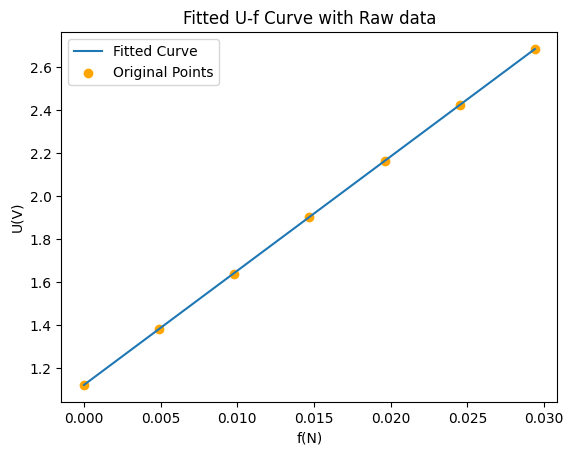
\includegraphics[width=0.5\textwidth]{picture1.png}
        \caption{力传感器标定曲线}
    \end{figure}

\end{enumerate}

\subsection{测量表面张力系数}

\begin{enumerate}
    \item 将待测液体倒入玻璃盘中,小心放入塑料容盘中,并一起放入水箱上室。
    \item 将力传感器转至容器内,挂上吊环,轻触吊环减小晃动。
    \item 关闭阀门,反复挤压气囊使上室内水面上升,当吊环下沿均与待测液体接触时,松开阀门,使水面缓慢下降。
    \item 观察吊环从液体中拉起的物理过程,示波器观察传感器输出的变化趋势。
    \item 在液膜破裂,传感器输出发生突变后,按下示波器“STOP”按钮,测量突变前后的电压值 \(U_1, U_2\),计算电压差 \(\Delta U\),根据标定系数换算拉力。
    \item 多次测量得到$\Delta U = 0.8231(V)$
    \begin{figure}[htbp]
        \centering
        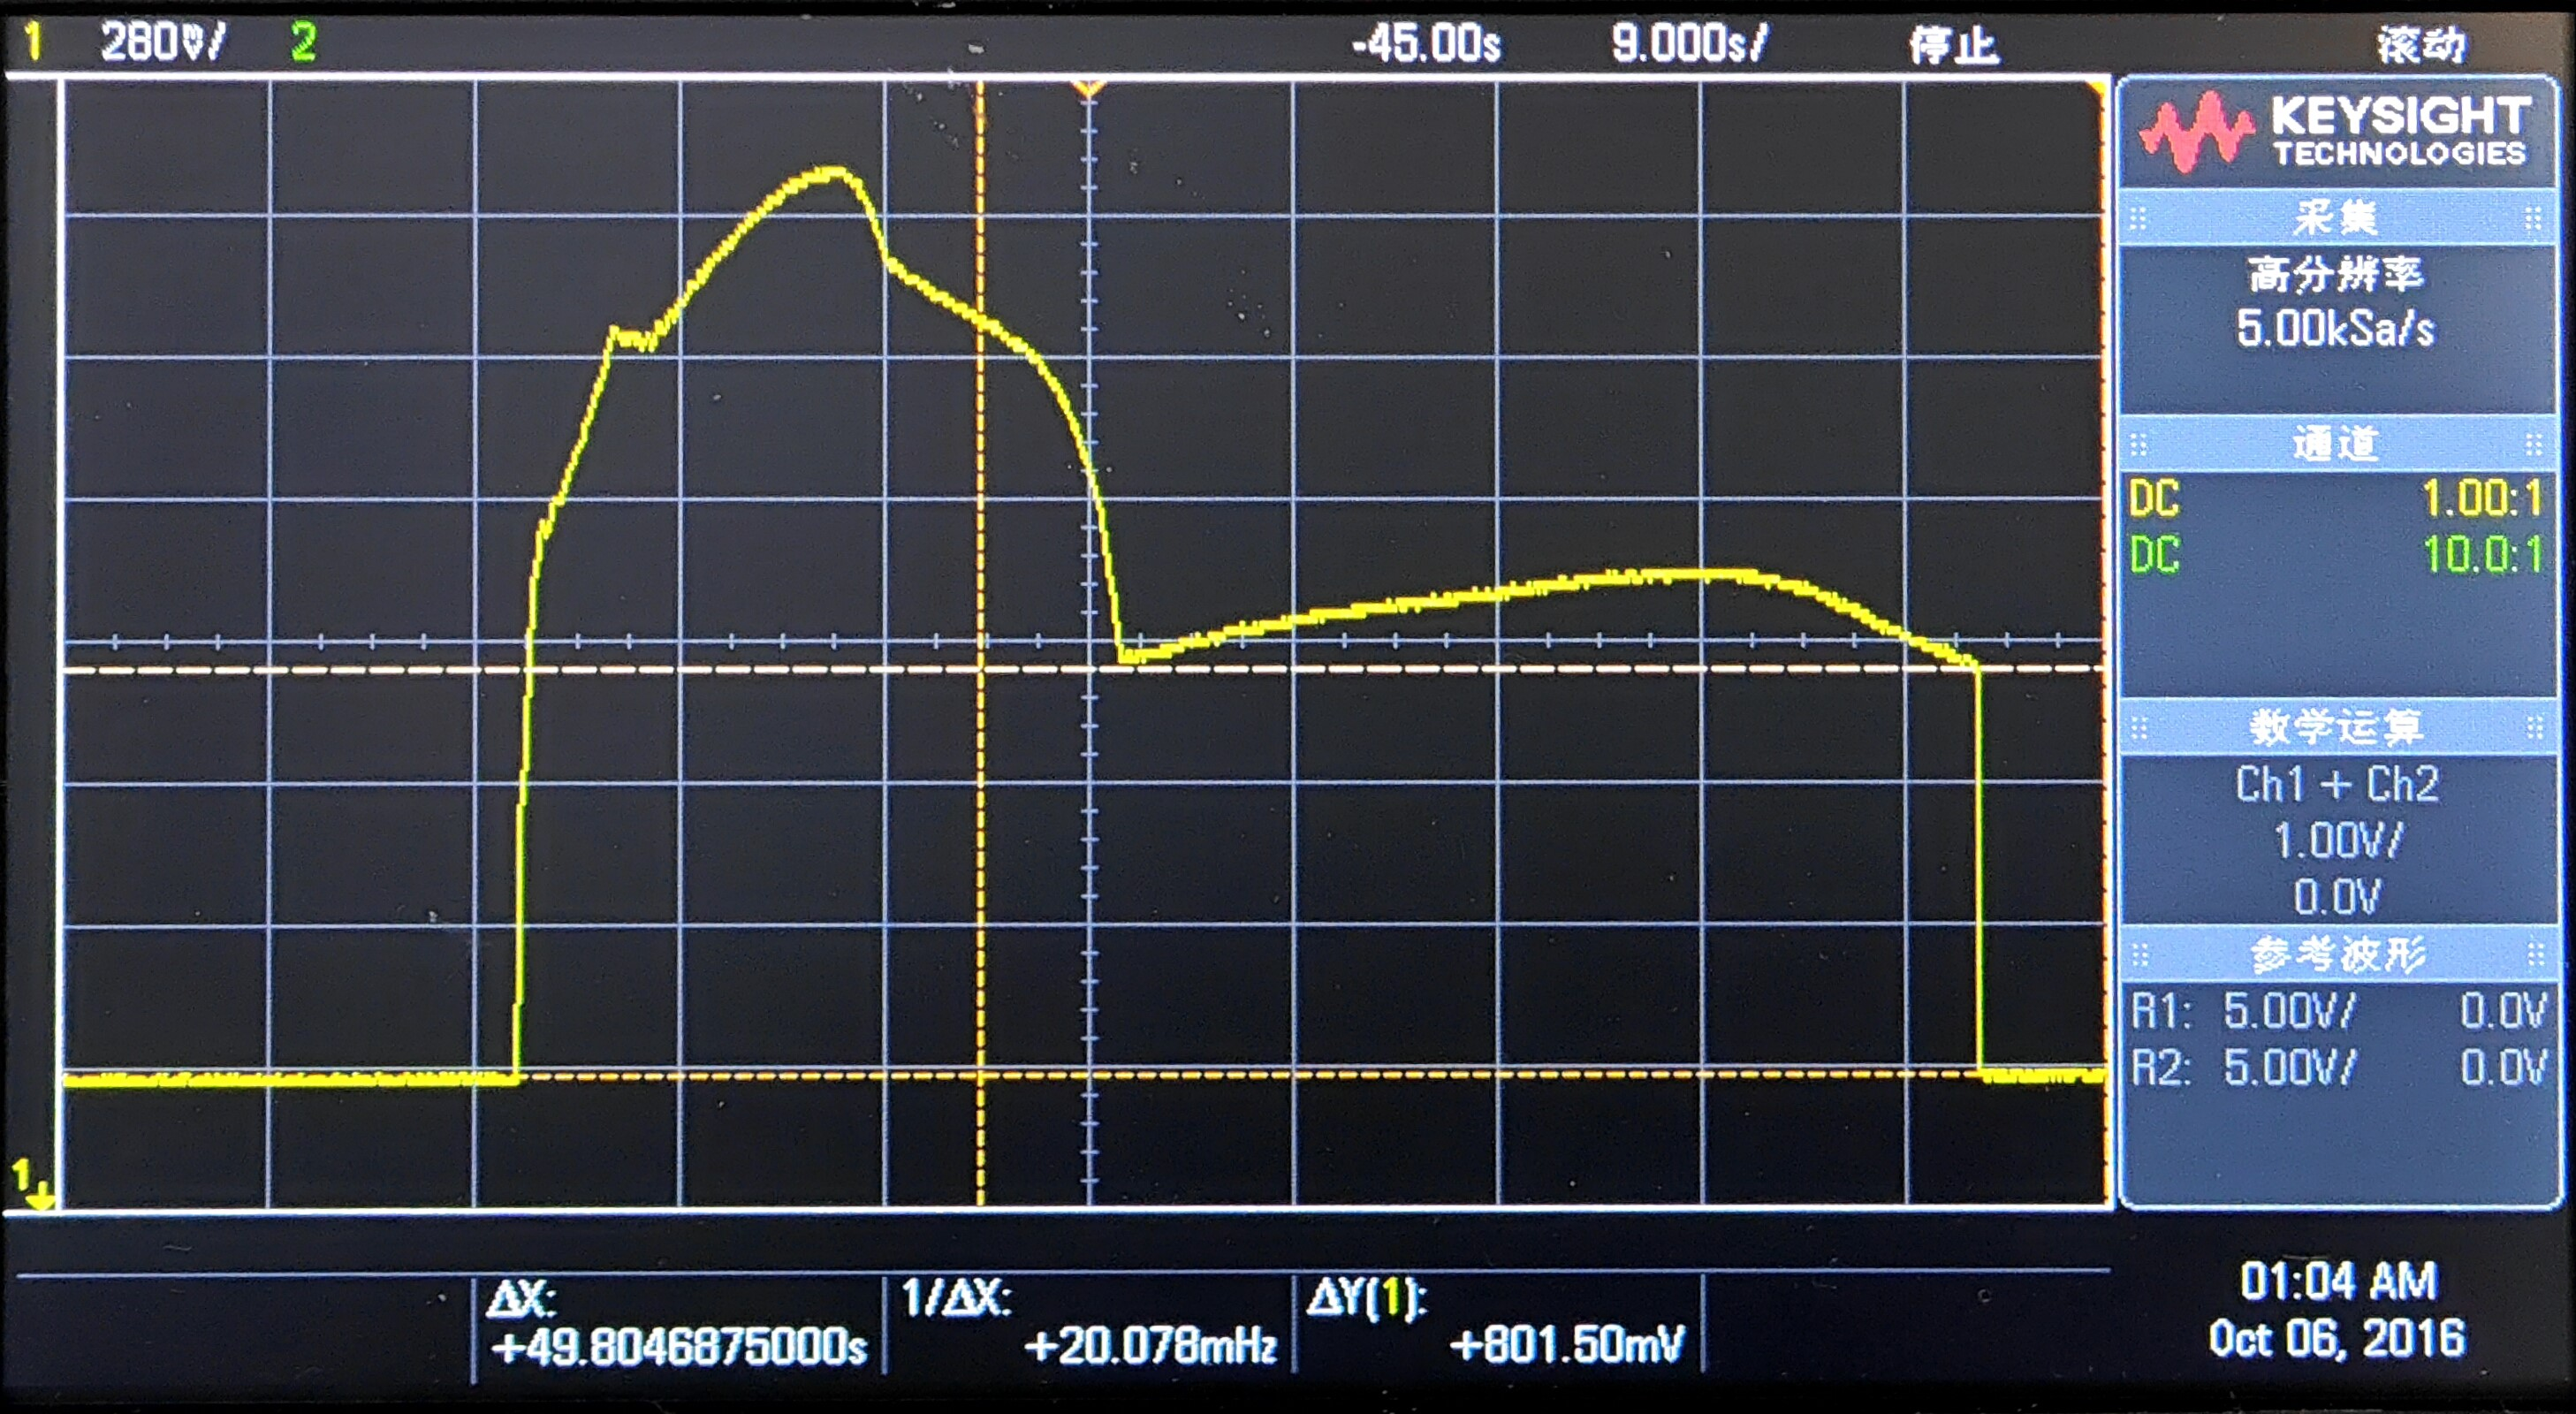
\includegraphics[width=0.5\textwidth]{fig.jpg}
        \caption{拉脱法测量表面张力系数电压曲线}
    \end{figure}
    \item 计算得到表面张力系数 $\sigma = 0.0725(N/m)$
\end{enumerate}


\end{document}
